\begin{definition}
Классом $\dtime{T(n)}$ называется класс языков, которые распознаются за время $O(T(n))$ детерминированной многоленточной машиной Тьюринга (МТ). Иными словами, время работы машины на любом слове длины $n$ не превосходит некоторой константы, умноженной на $T(n)$.
\end{definition}

TODO добавить NTIME

\begin{definition}
Язык $A$ сводится по Карпу к языку $B$ ($A \karp B$), если существует полиномиально вычислимая $f$ такая, что $x \in A \Longleftrightarrow f(x) \in B$.
\end{definition}

\begin{definition}
$A$ логарифмически сводится к $B$ ($A \lsv B$), если существует логарифмически вычислимая функция $f$ такая, что $x \in A \Longleftrightarrow f(x) \in B$.
\end{definition}

\subsection{\p}

\begin{definition}
$\p = \bigcup\limits_{c=1}^{\infty}\dtime{n^c}$

Другими словами, класс \p --- множество языков, распознающихся за полином от длины входа.
\end{definition}

\begin{note} 
\p замкнут относительно дополнений, объединений и пересечений, звезды Клини.
\end{note}

\subsection{\np}

\begin{definition}
Класс \np состоит в точности из тех языков $A$, для которых существует некая детерминированная МТ двух аргументов $V(x, s)$, работающая по времени за $poly(|x|)$ такая, что
$$
\forall x \in \Sigma^* \ x \in A \Longleftrightarrow \exists s: V(x, s) = 1.
$$
Тогда $V$~--- верификатор, а $s$~--- сертификат для данного $x$.
\end{definition}

\begin{definition}[Эквивалентное определение]
Классом $\ntime{T(n)}$ называется класс языков, которые распознаются за время $O(T(n))$ недетерминированной машиной Тьюринга (МТ). Иными словами, время работы машины на любом слове длины $n$ не превосходит некоторой константы, умноженной на $T(n)$.

$\np = \bigcup\limits_{c=1}^{\infty}\ntime{n^c}$
\end{definition}

\begin{note} 
\np замкнут относительно объединений, пересечений и звезды Клини, но не дополнений.
\end{note}

\subsection{\conp}

\begin{definition}
Класс \conp состоит в точности из тех языков $A$, для которых $\overline{A} \in \np$.
\end{definition}

\begin{statement}
$\p \subset \np \cap \conp$
\end{statement}

\begin{proof}
Вложение $\p \subset \np$ тривиально (детерминированная МТ является частным случаем недетерминированной МТ). Так как класс \p замкнут относительно дополнений, то и $\p \subset \conp$. 
\end{proof}

\begin{statement}
$\p = \np \Longleftrightarrow \p = \conp$. То есть все три класса равны, если верно хотя бы одно из утверждений.
\end{statement}

\begin{proof}
\p замкнут относительно дополнения, тогда и \np замкнут относительно дополнения, тогда $\conp \subset \np$. 
\end{proof}

\begin{note}
$\np \cap \conp$ замкнут относительно дополнений.
\end{note}

\begin{proof}
$A \in \np \cap \conp \Longrightarrow \overline{A} \in \conp \cap \np$. Пояснение. Если $A \in \np$, то по определению $\overline{A} \in \conp$. Аналогично рассмотреть, если $A \in \conp$
\end{proof}

\subsection{\npc (\np-полные)}

\begin{definition}
$A \in \nph$, если $\forall B \in \np \ B \karp A$.
\end{definition} 

\begin{statement}
Если $A \in \nph$ и $A \karp B$, то $B \in \nph$.
\end{statement}

\begin{statement}
Класс \npc (\textbf{NP-Complete}) состоит в точности из тех языков $A$, которые:
\begin{enumerate}
    \item $A \in \np$;
    \item $A \in \nph$.
\end{enumerate}
\end{statement}

\begin{statement}
Если $\p = \np$, то 
$\forall A \in \np \setminus \{\varnothing, \Sigma^*\} \ A \in \npc$.
\end{statement}

\begin{proof} получаем, что любой такой язык сводим по Карпу к любому другому из этого множества, то есть они все ещё и из \nph. Так как они все из \np, значит, они все и из \npc.
\end{proof}

% \begin{statement}[?]
% $\npc \cap \conp = \emptyset$
% \end{statement}

\subsection{\e}

\begin{definition}
$\e = \dtime{2^{O(n)}} = \bigcup\limits_{c = 1}^\infty \dtime{2^{cn}}$.
\end{definition}

\begin{note}
Очевидно, что
\begin{equation*}
    \p \subsetneq \e \subsetneq \EXP
\end{equation*}

Из теоремы об иерархии по времени следует, что все вложения строгие
\end{note}

\subsection{\EXP}

\begin{definition}
$\EXP = \bigcup\limits_{c = 1}^\infty \dtime{2^{n^c}}$.
\end{definition} 

\begin{note} Согласно теореме об иерархии по времени
\begin{equation*}
    \p \subseteq \np \subseteq \EXP
\end{equation*}
Более того, $\p \subsetneq \EXP$.
\end{note}

\subsection{\sk{k}}

\begin{definition}
Класс \sk{k} состоит из тех языков, для которых существует детерминированная МТ $V$, работающая по времени за $\text{poly}(|x|)$, при этом $x \in A \Longleftrightarrow \exists y_1 \forall y_2 \exists y_3 \ldots \ V(x, y_1, \ldots, y_k) = 1$.
\end{definition}

\subsection{\pk{p}}

\begin{definition}
Класс \pk{k} состоит из тех языков, для которых существует детерминированная МТ $V$, работающая по времени за $\text{poly}(|x|)$, при этом $x \in A \Longleftrightarrow \forall y_1 \exists y_2 \forall y_3 \ldots \ V(x, y_1, \ldots, y_k) = 1$.
\end{definition}

\subsection{\ph}

\begin{definition}
$\ph \textit{ (polynomial hierarchy)} = \bigcup\limits_{k = 0}^\infty \sk{k}$
\end{definition}

\begin{note}
Легко заметить, что $\sk{0} = \pk{0} = \p$.
\end{note}

\begin{note}
Тоже легко заметить, что $\sk{1} = \np$, $\pk{1} = \conp$.
\end{note}

\begin{statement}
$\sk{k} =$ \textbf{co}\pk{k}.
\end{statement}

\begin{proof}
Получим определение другого через отрицание определения.
\end{proof}

\begin{note}
Классы \sk{k} и \pk{k} замкнуты относительно объединения.
\end{note}

\begin{note}
$\sk{k} \cup \pk{k} \subset \sk{k + 1} \cap \pk{k + 1}$. Для этого можно добавить фиктивную переменную (сначала или с конца) и квантор по ней. Отсюда следует, что $\ph = \bigcup\limits_{k = 0}^\infty \pk{k}$.
\end{note}

\subsection{\sk{k}-полные}

\subsection{\pk{k}-полные}

\begin{definition}
Определения обоих классов аналогичны определению \npc (сводимость та же, по Карпу).
\end{definition}

\begin{note}
Подмножества соответствующих \sk{k} или \pk{k}.
\end{note}

\subsection{\skp{k}}

\subsection{\pkp{k}}

\begin{definition}
Альтернирующая машина Тьюринга --- машина Тьюринга с многозначной функцией перехода, у которой все состояния делятся на два класса: $\Sigma$-состояния и $\Pi$-состояния, а все конфигурации либо принимающие, либо отвергающие. Определяем рекурсивно: если конфигурация содержит принимающее состояние, то она принимающая. Если конфигурация содержит $\Sigma$-состояние ($\Pi$-состояние), то она принимающая, если хотя бы один из ее сыновей (все сыновья) принимающий. Аналогично определяется отвергающее состояние.
\end{definition}

\begin{definition}
Класс $\atime{t(n)}$ — класс языков, для которых найдётся альтернирующая МТ такая, что все её ветви имеют длину $O(t(|x|))$ и $x \in A$ равносильно тому, что начальное состояние принимающее.
\end{definition}

\begin{note} Внимательный читатель уже мог заметить, что граф вычислений альтернирующей машины Тьюринга является графом игры с выигрышными и проигрышными состояниями. Если состояние принимающее, тогда из $\Sigma$-состояний ($\exists$-состояний) ходит первый игрок, а из $\Pi$-состояний ($\forall$-состояний) ходит второй.
\end{note}

\begin{note} Если в предыдущем замечании ограничить число ходов, то можно получить классы $\sk{k}$ ($\pk{k}$) как множество выигрышных позиций для первого (второго) игрока.
\end{note}

\begin{definition}
Класс $\sktime{k}{t(n)}$~--- подкласс $\atime{t(n)}$, в котором стартовое — $\Sigma$-состояние ($\exists$-состояние), а количество перемен вида состояния на любой ветке не превысит $k - 1$.
\end{definition}

\begin{definition}
Класс $\pktime{k}{t(n)}$~--- подкласс $\atime{t(n)}$, в котором стартовое — $\Pi$-состояние ($\forall$-состояние), а количество перемен вида состояния на любой ветке не превысит $k - 1$.
\end{definition}

\begin{definition}
$\skp{k} = \bigcup\limits_{c = 1}^\infty \sktime{k}{n^c}$
\end{definition}

\begin{definition}
$\pkp{k} = \bigcup\limits_{c = 1}^\infty \pktime{k}{n^c}$
\end{definition}

\begin{theorem}
$\sk{k} = \skp{k}$ и $\pk{k} = \pkp{k}$
\end{theorem}

% \begin{note} Если в предыдущем замечании ограничить число ходов, то можно получить классы $\sk{k}$ ($\pk{k}$) как множество выигрышных позиций для первого (второго) игрока.
% \end{note}

\begin{note} Получается такая цепочка вложенностей:
$$
\lsp \subseteq \rl \subseteq \nlsp = \conlsp \subseteq \p \subseteq \np \subseteq \ph \subseteq \psp = \npsp = \ap \subseteq \EXP \subseteq \cdots
$$

Но $\lsp \ne \psp$ и $\p \ne \EXP$.
\end{note}

\subsection{\psp}

\begin{definition}
Классом $\dsp{S(n)}$ называется класс языков, которые распознаются детерминированными МТ на $O(S(n))$ памяти.
\end{definition}

\begin{definition}
$\psp = \bigcup\limits_{c = 1}^\infty \dsp{n^c}$.
\end{definition}

\begin{note}
$\psp \subseteq \EXP$.
\end{note}

\begin{note}
$\ph \subseteq \psp$ (для каждого \sk{k} можно построить необходимую машину, перебирающую все переменные под кванторами (и помнящую только последнее значение, которое перебрали)).
\end{note}

\begin{note}
$\p \subseteq \np \subseteq \ph \subseteq \psp \subseteq \EXP$, но $\p \subsetneq \EXP$.
\end{note}

\subsection{\npsp}

\begin{definition}
Пусть $M$~--- МТ с неизменяемой входной лентой. Пусть количество ячеек, измененных при обработке $x$ не превосходит $O(S(|x|))$. Тогда $M$ использует $S(n)$ памяти. 
\end{definition}

\begin{definition}
Классом $\nsp{S(n)}$ называется класс языков, которые распознаются недетерминированными МТ на $O(S(n))$ памяти.
\end{definition}

\begin{definition}
$\npsp = \bigcup\limits_{c = 1}^\infty \nsp{n^c}$.
\end{definition}

\begin{theorem}[Сэвич]
$\nsp{S(n)} \subset \dsp{S(n)^2}$
\end{theorem}

\begin{corollary}
$\npsp = \psp$
\end{corollary}

\subsection{\psp-полные}

\begin{definition}
Определение аналагично \npc (сводимость та же, по Карпу).
\end{definition}

\subsection{\ap}

\begin{definition}
$\ap = \bigcup\limits_{c = 1}^\infty \atime{n^c}$.
\end{definition}

\begin{theorem}
$\ap = \psp$
\end{theorem}

\subsection{\lsp}

\begin{definition}
Пусть S(n) — неубывающая функция. Классом $\dsp{S(n)}$ называется класс языков, которые можно распознать на детерминированной
машине Тьюринга, на любом входе длины $n$ использующей $O(S(n))$ ячеек на рабочих лентах.

$\lsp = \dsp{\log n}$.
\end{definition}

\begin{note}
$\lsp \neq \psp$
по теореме об иерархии по памяти
\end{note}

\subsection{\nlsp}

\begin{definition}
$\nlsp = \nsp{\log n}$.
\end{definition}

\begin{note} $\lsp \subseteq \nlsp \subseteq \p$. Первое вложение тривиально, второе следует из теоремы о связях пространственно-временных классов. Ни про одно из вложений не известно на данный момент, строгое ли оно.% Однако известно, что $\lsp \neq \p$. --- НЕТ!
\end{note}

\begin{theorem}[О связях пространственно-временных классов (7.5 в compl-book)]
Имеют место соотношения
$$
\dtime{t(n)} \subset \ntime{t(n)} \subset \dsp{t(n)} \subset \nsp{t(n)} \subset \dtime{2^{O(t(n))}}
$$

Последняя запись означает $\bigcup_{c = 0}^{\infty} \dtime{2^{ct(n)}}$.
\end{theorem}

\subsection{\nlcsp (\nlsp-полные)}

\begin{definition} Логарифмическая вычислимость может определяться 2мя способами:
\begin{enumerate}
    \item Есть входная лента только для чтения, рабочая лента и выходная только для записи ответа слева направо. Должна быть программа, получающая $x$ на входной ленте, записывающая $f(x)$ на выходной ленте и использующая $O(log(n))$ ячеек на рабочей ленте.
    \item $|f(x)| = poly(|x|)$, $\{(x,i)\ |\ |f(x)| \le i\} \in \lsp$ и $\{(x,i)\ |\ (f(x))|_i = 1 \} \in \lsp$.
\end{enumerate}
\end{definition}

\begin{definition}
$A$ — \textbf{NL-hard}, если к нему можно свести все языки из \nlsp.
\end{definition} 

\begin{definition}
$A \in \nlcsp$, если $A \in \nlsp$ и $A$ из \textbf{NL-hard}.
\end{definition}

\begin{note}
Очевидно, что $\nlcsp \subset \nlsp$.
\end{note}

\subsection{\conlsp}

\begin{definition}
$A \in \conlsp \Longleftrightarrow \overline{A} \in \nlsp$
\end{definition}

\begin{theorem}[Иммермана-Селепченьи]
$\nlsp = \conlsp$.
\end{theorem}

\subsection{$\ppoly$}

\begin{definition}
$\ppoly$ ~--- класс языков, распознаваемых схемами полиномиального размера (не глубины, а именно число элементов).
\end{definition}

\begin{statement}
$\p \subsetneq \ppoly$
\end{statement}

\begin{proof}
Доказательство в целом повторяет доказательство теоремы Кука–Левина. А именно, если есть машина Тьюринга, работающая за $p(n)$ шагов, то строится схема размера $O(p(n)^2)$, моделирующая работу этой машины. Схема будет вычислять символы, стоящие в протоколе работы этой машины. Поскольку каждый символ зависит только от 4 символов на предыдущем этапе, эту зависимость можно выразить булевой функцией фиксированного размера, которая записывается в виде схемы. Таким образом, можно вычислить эле- менты всех ячеек протокола, а затем проверить, что в последней строке есть принимающее состояние.
\end{proof}

\begin{statement}
$\p \neq \ppoly$
\end{statement}

\begin{proof}
Например, в $\ppoly$ будет лежать любой \textit{унарный} язык $U$, т.е. язык, содержащий только слова вида $1^k$. Действительно, для каждой длины $U \cap \{0, 1\}^k$ будет либо пустым множеством, либо состоять только из $1^k$. В первом случае язык распознаётся тождественно ложной схемой, во втором --- конъюнкцией.

А унарные языки могут быть даже неразрешимыми, например $\uhalt = \{1^k | $ машина Тьюринга $M_k$ останавливается на входе $k$\}. Также они могут быть разрешимыми, но не лежать в $\p$. Например, можно взять любой язык $A \in \textbf{EEXP} \setminus \EXP$ (такой есть по теореме об иерархии) и рассмотреть ${1^k | k \in A}$. Если его можно распознать за полиномиальное время, то $A$ можно распознать за экспоненциальное время, что противоречит выбору $A$.
\end{proof}

\begin{theorem}[Карпа-Липтона]
Если $\np \subset \ppoly$, то $\ph = \sk{2}$.
\end{theorem}

\begin{theorem}[Мейера]
Если $\EXP \subset \ppoly$, то $\EXP = \sk{2}$.
\end{theorem}

\begin{note}
В условиях теоремы выше верно, что $\p \ne \np$, так как иначе $\p = \sk{2} = \EXP$, что неверно по теореме об иерархии.
\end{note}

\subsection{\acd{d}}

\begin{definition}
Классом \acd{d} называется класс языков, распознаваемых схемами полиномиального размера глубины $O(\log^d n)$, в которых входящая степень всех вершин, помеченных $\lor$ и $\land$ произвольная.
\end{definition}

\subsection{\ncd{d}}

\begin{definition}
Классом \ncd{d} называется класс языков, которые разпознаются семейством схем полиномиального размера и глубины $O(\log^d n)$, в которых элементы $\lor$ и $\land$ имеют входящую степень ровно 2.
\end{definition}

\subsection{\nc}

\begin{definition}
$\nc = \bigcup\limits_{d=0}^\infty \ncd{d}$.
\end{definition}

\begin{statement}
Для всех $d$ выполнено $\ncd{d} \subset \acd{d} \subset \ncd{d+1}$.
\end{statement}

\begin{proof}
Заметим, что схемы для \ncd{d} --- это частный случай схем для \acd{d}, отсюда берётся первое включение. Если же элемент $\lor$ или $\land$ имеет входную степень $k$, то можно его заменить двоичным деревом глубины $\ceil{\log k}$ из элементов входной степени 2. Поскольку размер всей схемы был полиномиальным, такой же будет и максимальная входная степень каждого элемента, откуда $\ceil{\log k} = O(\log n)$. Таким образом, замена на двоичные деревья увеличит глубину не больше, чем в $O(\log n)$ раз, т.е. из $O(\log^d n)$ она превратится в $O(\log^{d+1} n)$. Таким образом, $\acd{d} \subset \ncd{d+1}$.
\end{proof}

\begin{note} Отсюда получается, что $\bigcup\limits_{d=1}^\infty \acd{d} = \bigcup\limits_{d=1}^\infty \ncd{d} = \nc$, поэтому отдельного обозначения \textbf{AC} не вводят.
\end{note}

\begin{statement}
$\ncd{0} \neq \acd{0}$.
\end{statement}

\begin{proof}
В классе \ncd{0} лежат языки, которые вычисляются схемами константной глубины $c$. Поскольку у каждого элемента не больше  двух входов, число изначальных входов, от которых зависит значение, будет не больше $2^c$. Поэтому такой схемой нельзя вычислить функцию, которая зависит от всех входов, например, их конъюнкцию. В то же время конъюнкция тривиальным образом лежит в \acd{0}, откуда $\ncd{0} \neq \acd{0}$.
\end{proof}

\begin{theorem}
$\acd{0} \neq \ncd{1}$.
\end{theorem}

\textbf{Идея доказательства.} Рассмотрим язык

$$\textbf{PARITY} = \{\{x_1, \ldots, x_n\} : \bigoplus\limits_{i=1}^n x_n = 1\}$$

Покажем, что \mbox{$\textbf{PARITY} \in \ncd{1}$} и $\textbf{PARITY} \not\in \acd{0}$.

\begin{itemize}
    \item \underline{$\textbf{PARITY} \in \ncd{1}$.} Нужно зафиксировать схему для $\oplus$ и собрать из таких схем двоичное дерево.
    \item \underline{$\textbf{PARITY} \not\in \acd{0}$.} Доказывается алгебраической техникой: показывается, что любой язык из \acd{0} можно хорошо приблизить некоторым многочленом, а \textbf{PARITY} --- нельзя.
\end{itemize}

\begin{theorem}[8.26 в compl-book]
$$
\nlsp \subset \acd{1}
$$
\end{theorem}

\subsection{\bpp}

\begin{definition} Классом \bpp (bounded-error probabilistic polynomial) называется класс языков $A$, для которых существует полиномиальный в худшем случае вероятностный алгоритм $V$, такой что:

\begin{itemize}
    \item если $x \in A$, то $\Pr_r[V(x, r) = 1] \geq \frac{2}{3}$;
    \item если $x \not\in A$, то $\Pr_r[V(x, r) = 1] \leq \frac{1}{3}$.
\end{itemize}
\end{definition}

\begin{definition}
В силу симметричности определения, если $A \in \bpp$, то и $\overline{A} \in \bpp$, то есть $\mathbf{coBPP} = \bpp$.
\end{definition}

\begin{statement}
$\bpp \subset \psp$.
\end{statement}

\begin{proof} На полиномиальной памяти можно найти количество таких $r$ (полиномиальной длины в силу определения \bpp), что $V(x, r) = 1$, посчитать вероятность и сравнить её с $\frac{1}{3}$ и $\frac{2}{3}$.
\end{proof}

\begin{theorem}[Эйдлмана]
$$
\bpp \subset \ppoly
$$
\end{theorem}

\begin{theorem}[Сипсер–Гач–Лаутеман]
$$
\bpp \subset \Sigma_2^p \cap \Pi_2^p
$$
\end{theorem}

\begin{corollary}
Если $\p = \np$, то $\p = \bpp$
\end{corollary}

\subsection{\rp}

\begin{definition}
Классом \rp (randomized polynomial) называется класс языков $A$, для которых существует полиномиальный в худшем случае вероятностный алгоритм $V$, такой что:

\begin{itemize}
    \item если $x \in A$, то $\Pr_r[V(x,r) = 1] \geq \frac{1}{2}$;
    \item если $x \not\in A$, то $\Pr_r[V(x,r) = 1] = 0$.
\end{itemize}
\end{definition}

\begin{statement}
$\rp \subset \np$.
\end{statement}

\begin{proof} Альтернативное определение $A \in \np$ через сертификаты и вероятность:

\begin{itemize}
    \item если $x \in A$, то $\Pr_r[V(x,r) = 1] > 0$;
    \item если $x \not\in A$, то $\Pr_r[V(x,r) = 1] = 0$.
\end{itemize}

То есть, любое значение $r$ (в контексте \np сертификата), при котором $V(x, r) = 1$, будет доказательством того, что $x \in A$.
\end{proof}

\subsection{\corp}

\begin{definition}
Классом \corp называется класс языков $A$, для которых существует полиномиальный в худшем случае вероятностный алгоритм $V$, такой что:

\begin{itemize}
    \item если $x \in A$, то $\Pr_r[V(x,r) = 1] = 1$;
    \item если $x \not\in A$, то $\Pr_r[V(x,r) = 1] \leq \frac{1}{2}$.
\end{itemize}
\end{definition}

\begin{note}
Если $A \in \rp$, то $\overline{A} \in \corp$.
\end{note}

\begin{statement}
$\corp \subset \conp$.
\end{statement}

\begin{proof}
 Альтернативное определение $A \in \conp$ через сертификаты и вероятность:

\begin{itemize}
    \item если $x \in A$, то $\Pr_r[V(x,r) = 1] = 1$;
    \item если $x \not\in A$, то $\Pr_r[V(x,r) = 1] < 1$.
\end{itemize}

То есть, если для любого значения $r$ (в контексте \conp сертификата) верно $V(x, r) = 1$, то $x \in A \in \conp$.
\end{proof}

\subsection{\zpp}

\begin{definition}
Классом \zpp (zero-error probabilistic polynomial) называется множество языков $A$, для которых существует вероятностный алгоритм $V$, такой что $x \in A$ при всех $r$ эквивалентно $V(x, r) = 1$, а для каждого $x$ ожидаемое по $r$ время работы полномиально.
\end{definition}

\begin{statement}
$\zpp = \rp \cap \corp$
\end{statement}

\begin{proof}
Пусть $A \in \zpp$. Докажем, что $A \in \rp$. Пусть $U$ --- алгоритм, распознающий $A$ и работающий в среднем за $p(n)$. Рассмотрим такой алгоритм: запустить $U$ на $2p(n)$ шагов. Если он закончил работу, вернуть тот же ответ, иначе вернуть 0. Если $x \not \in A$, то в любом случае будет возвращён 0. Если же $x \in A$, то по неравенству Маркова с вероятностью не меньше $\frac{1}{2}$ алгоритм закончит работу и потому ответ будет 1. Значит, $A \in \rp$. Вложение $A \in \corp$ доказывается аналогично, нужно только при отсутствии ответа вместо 1 возвращать 0.

Обратно, пусть $A \in \rp \cap \corp$. Пусть $V$ --- алгоритм, не допускающий ошибок первого рода (такой есть, т.к. $A \in \rp$), а $W$ --- не допускающий ошибок второго рода (такой есть, т.к. $A \in \corp$). Запустим алгоритм $V$ на входе $x$ Если он вернул 1, то заведомо $x \in A$. Иначе запустим $W(x)$. Если он вернул 0, то заведомо $x \not \in A$. Так будем повторять со свежими случайными битами, пока не получим $V(x) = 1$ или $W(x) = 0$. Вероятность получения ответа на каждой стадии не меньше $\frac{1}{2}$, поэтому ожидаемое число стадий не больше 2. Значит, $A \in \zpp$. Заметим, что при таком алгоритме не исключены бесконечные ветви, хотя они и возникают с нулевой вероятностью. В базовом определении вероятностной машины они были запрещены, и их действительно можно избежать: после полиномиального числа стадий вероятность отсутствия ответа станет экспоненциально малой, и можно в этом случае запустить экспоненциальный алгоритм.

\end{proof}

\subsection{\pp}

\begin{definition}
Классом \pp называется класс языков $A$, для которых существует полиномиальный в худшем случае вероятностный алгоритм $V$, такой что:

\begin{itemize}
    \item если $x \in A$, то $\Pr_r[V(x,r) = 1] \geq \frac{1}{2}$;
    \item если $x \not\in A$, то $\Pr_r[V(x,r) = 1] < \frac{1}{2}$.
\end{itemize}
\end{definition}

\begin{note} В итоге получится такой граф вложенностей:

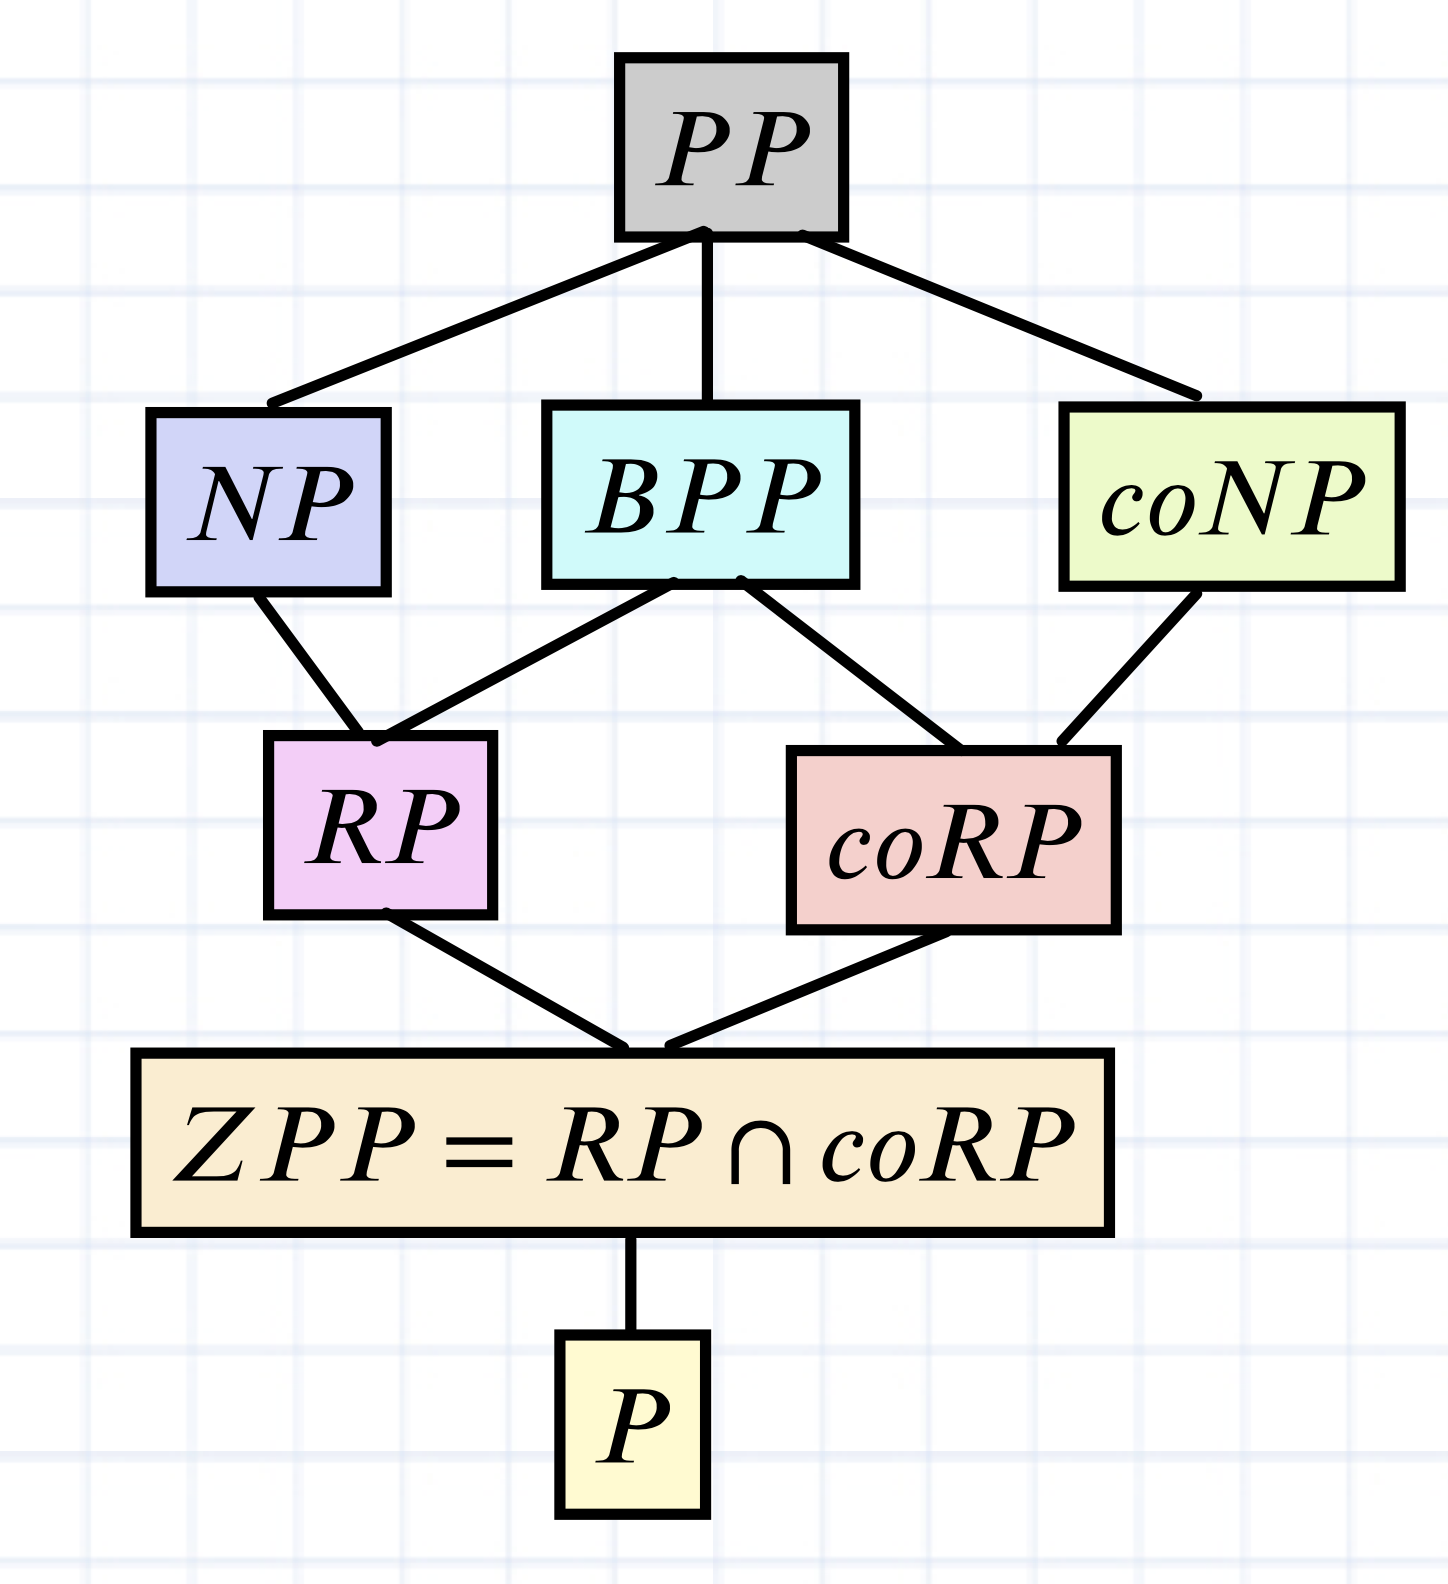
\includegraphics[scale=0.2]{images/PP_class.png}

\end{note}

\begin{statement}
$\pp \subset \psp$.
\end{statement}

\begin{proof} Доказывается аналогично вложению $\bpp 
\subset \psp$: нужно найти долю $r$ таких, что $V(x, r) = 1$ и сравнить её с $\frac{1}{2}$.
\end{proof}

\begin{statement}
$\np \cup \conp \subset \pp$
\end{statement}

\begin{proof}
Для $\np$ достаточно применить лемму для $m(x) = 1$.
Результат для $\conp$ получается из замкнутости относительно дополнения.
\end{proof}

\begin{lemma}[10.11 в compl-book]
Пусть $V$ --- полиномиальный верификатор с длиной сертификата $p(n)$. Пусть функция $m$ вычислима за полиномиальное время и принимает целые значения от 0 до $2^{p(n)}$. Тогда существует другой полиномиальный верификатор $W$ с длиной сертификата $q(n)$, такой что если $\#_V(x) \geq m(x)$, то $\#_W(x) > \frac{1}{2} 2^{q(n)}$, а если $\#_V(x) < m(x)$, то $\#_W(x) < \frac{1}{2} 2^{q(n)}$.
\end{lemma}

\begin{note}
$\ph \subset \pp$ -- открытый вопрос.
\end{note}

\subsection{\rclass (разрешимые)}

\begin{definition}
\rclass — множество всех разрешимых языков, то есть тех, для которых есть машина Тьюринга, способная их разрешить (проверить $x \in A$).
\end{definition} 

Давайте задумаемся о том, что может быть в нём. Так как в \rclass нет ограничения на время и память, то в принципе почти все пройденные классы там лежат, ведь в определении почти всех классов  предполагалось наличие какой-то машины Тьюринга разрешающей язык.

Но вот, например, в $\ppoly$ есть неразрешимый язык — $\uhalt$, поэтому $\ppoly \not\subset \rclass$.

\begin{definition}
$\uhalt = \{1^k \ | \text{ МТ $M_k$ остановится на входе $k$}\}$.
\end{definition}

\subsection{\re (перечислимые)}

\begin{definition}
\re~--- множество всех перечислимых языков, для которых есть МТ, способная перечислить все слова из него, причем каждое за конечное время (при этом для слов не из языка может зациклиться).
\end{definition}

Вроде как тривиально, что $\rclass \subset \re$. Но можно сказать и большее, $\rclass \subsetneq \re$, так как неразрешимый $\uhalt \in \re$, то есть $\uhalt \in \re \setminus \rclass$.

\subsection{Приложение}

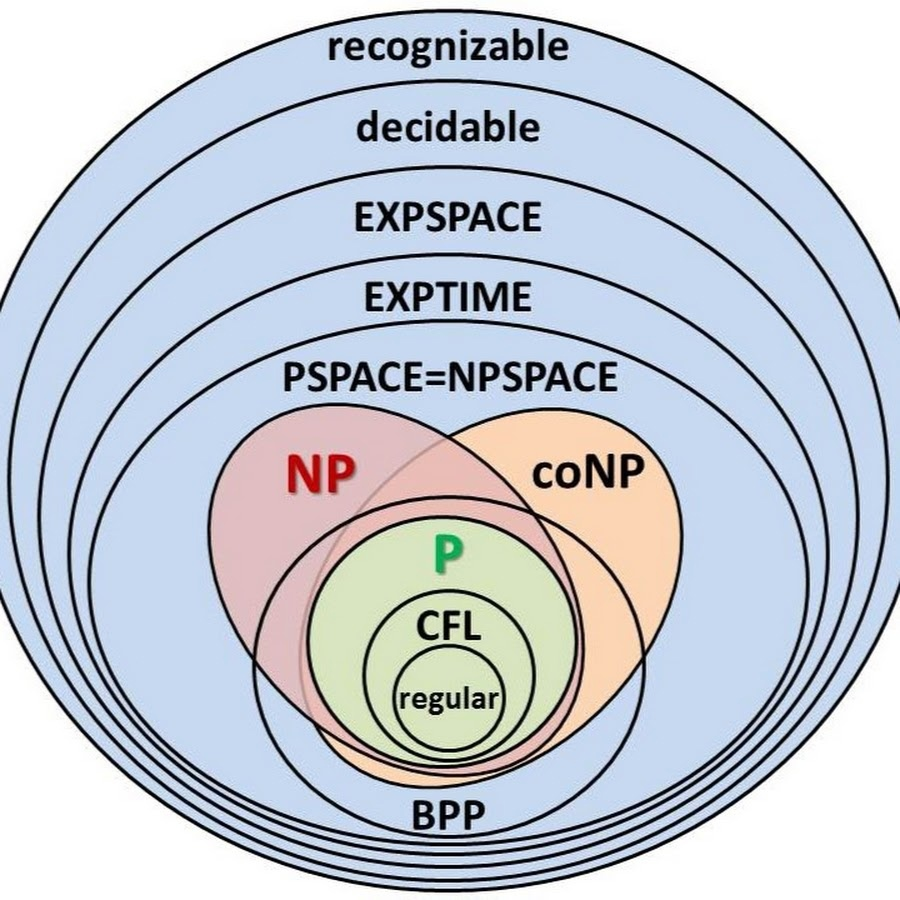
\includegraphics[scale=0.25]{images/classes.jpeg}